\begin{para}{Функция расстояния}

$dist = \alpha dist_{categorical} + (1 - \alpha)dist_{numeric}$

$dist_{categorical}$ - количество свойств, которые не совпадают

$dist_{numeric} = euclidean | manhattan$


\end{para}

\begin{para}{Зависимость F-меры от числа ближайших соседей}

\begin{figure}[h]
\center{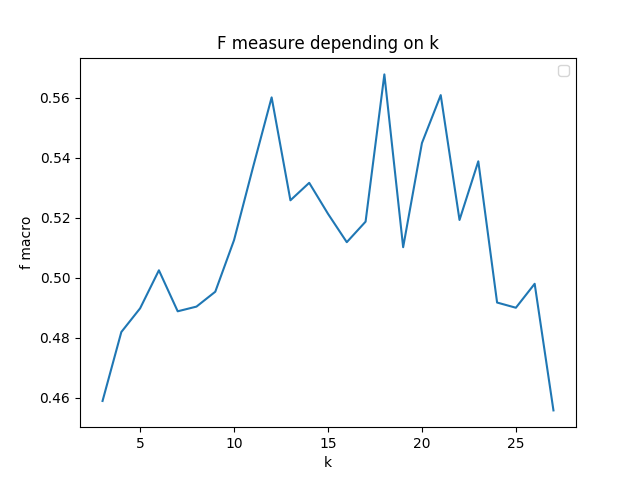
\includegraphics[width=1\linewidth]{f_measure_from_k}}
\label{ris:f_measure_from_k}
\end{figure}

\end{para}

\begin{para}{Зависимость F меры от ширины окна}

\begin{figure}[h]
\center{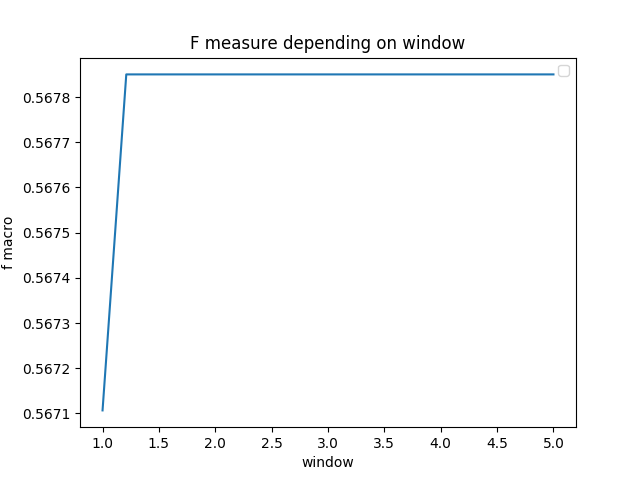
\includegraphics[width=1\linewidth]{f_measure_from_window}}
\label{ris:f_measure_from_window}
\end{figure}

\end{para}